% ----------------------------------------------------------------
% achemso --- Support for submissions to American Chemical
%  Society journals
% Maintained by Joseph Wright
% E-mail: joseph.wright@morningstar2.co.uk
% Originally developed by Mats Dahlgren
%  (c) 1996-98 by Mats Dahlgren
%  (c) 2007-2008 Joseph Wright
% Released under the LaTeX Project Public license v1.3c or later
% See http://www.latex-project.org/lppl.txt
% 
% Part of this bundle is derived from cite.sty, to which the
% following license applies:
%   Copyright (C) 1989-2003 by Donald Arseneau
%   These macros may be freely transmitted, reproduced, or
%   modified provided that this notice is left intact.
% ----------------------------------------------------------------
% 
% The achemso bundle provides a LaTeX class file and BibTeX style
% file in accordance with the requirements of the American
% Chemical Society.  The files can be used for any documents, but
% have been carefully designed and tested to be suitable for
% submission to ACS journals.
% 
% The bundle also includes the natmove package.  This package is
% loaded by achemso, and provides automatic moving of superscript
% citations after punctuation.

\documentclass[
%journal=ancac3, % for ACS Nano
%journal=acbcct, % for ACS Chem. Biol.
journal=jacsat, % for undefined journal
manuscript=article]{achemso}

\usepackage[version=3]{mhchem} % Formula subscripts using \ce{}
\usepackage{amsmath}
\usepackage{amssymb}
\usepackage{amsthm}

\newcommand*{\mycommand}[1]{\texttt{\emph{#1}}}

\author{Sammy M. Shaker}
\author{Nicholas Petkovich}
\author{Andreas Stein}
\email{a-stein@umn.edu}
\affiliation[University of Minnesota]
{Department of Chemistry, University of Minnesota Twin Cities, Minneapolis, Minnesota, }



\title[\texttt{achemso} demonstration]
{Silica and Vanadia Gardens: Studies in Structure, Morphology and Templating Porosity}

\begin{document}

\begin{abstract}
Silica gardens are an elementary example of an amorphous structure formed by ion exchange across a semipermeable membrane. In an attempt to template mesoporosity onto the structure of said gardens, a liquid-crystal templating method was used utilizing cetyltrimethylammonium bromide (CTAB) as a solute in silicate solution. While these attempts were unsuccessful, the morphology of the gardens was found to be heavily dependent upon the density of the solution. Additionally, gardens grown using salts and solutions of opposite acidity/basicity to those of the standard garden were explored, as well as gardens grown in vanadia solution.
\end{abstract}


\section*{Introduction}
First observed by Johann Rudolf Glauber in 1646, silica or chemical gardens are simple structures that illustrate spontaneous inorganic partitioning of chemical systems~\cite{Glauber}. A silica garden is formed by placing a transition metal salt into a solution of sodium silicate. In doing so, a layer of insoluble metal silicates and hydroxides forms at the salt-solution interphase, while water flows into the area containing the salt crystal. Thus, the system has partitioned itself into an area of a basic solution, the sodium silicate, (pH $\approx$ 11.5) and an area of acidic solution, the metal salt solution. This partitioning encourages the transfer of water and sodium ions into the metal salt solution, which helps shape the silica garden into what would become its final structure. At the point in which the garden has stopped growing, the pH in both the solution outside of the silica garden and that inside the silica garden is approximately 11.5, and the system is in dynamic equilibrium~\cite{Kunz}. The structure of the metal silicate is amorphous and shows no regular structure without outside interference. 

Here, we present an attempt to form a mesoporous silica garden using liquid-crystal templating with cetyltrimethylammonium bromide (CTAB), a cationic surfactant. When these attempts were unsuccessful, as shown by small angle x-ray scattering (SAXS) measurements, the rate of growth was slowed by utilizing an acidic silica solution and a basic metal salt, but the identity of the structure formed was difficult to distinguish from a garden formed by selective precipitation. An attempt to incorporate a metal oxide into the structure of the 

In the course of our investigations, it became apparent that the behavior of the silica garden system had little to do with the silicate anions; rather, the presence of anions that formed an insoluble transition metal complex in an otherwise clear solution was one of the driving forces behind the formation of the gardens. As such, we present the vanadia garden system, in which a transition metal salt was placed into a solution of sodium vanadate and subsequently formed a structure we name the "Vanadia Garden". We explored the effects of changing solution pH, mass of salt, and identity of salt on the structure of these gardens was subsequently explored.

\section*{Materials and Methods}
\textbf{Preparation of Sodium Silicate Garden} To prepare 1 M sodium silicate solution, 476 mL of 37 wt\% sodium silicate solution (Sigma-Aldrich Inc.) was combined with 24 mL of deionized water. The resulting solution was a 6 M solution. Then, 3 mL of this solution was combined with 15 mL of deionized water to form a 1 M sodium silicate solution. A pellet of praseodymium chloride hydrate (Alfa Aesar, 99\%) was formed by pressing .2 g of salt at 9 tonnes of pressure for 40 seconds. The pellet was then placed in the 1 M sodium silicate solution in a scintillation vial (Research Products Inc.) and sealed for 24 hours. Differing molarities, where prepared, followed the same general procedure with adjustments towards the amount of silicate necessary.
~\\
\textbf{Templating Porosity} To introduce the surfactant CTAB into the sodium silicate solution, the procedure above was followed with the variation that the sodium silicate was combined with 15 mL of deionized water and CTAB (Alfa Aesar, 99\%), in the desired concentration. The masses of CTAB corresponding to the final concentrations in solution were shown below: \\
\begin{center}
    \begin{tabular}{| l | l |}
    \hline
    Mass of CTAB (g) & Concentration in Solution (M)\\ \hline
    .656 & .1 \\ \hline
    1.31 & .2  \\ \hline
    1.97 & .3  \\ \hline
    2.62 & .4  \\ \hline
    3.28 & .5  \\ \hline
    3.94 & .6  \\ \hline
    4.60 & .7  \\ \hline
    5.24 & .8  \\ \hline
    \end{tabular}
\end{center} 
To dissolve the amount of CTAB required to make a specific concentration, stirring and heating at 40$^{\circ}$C may be necessary, and once dissolved gardens should be kept at approximately 40$^{\circ}$C to maintain dissolution of CTAB. \\
\textbf{Preparation of Backwards Silicate Garden} 
To prepare a backwards silicate garden, one must prepare a solution of 5 grams of ethanol (Sigma-Aldrich Inc., 99\%), 3 grams of tetraethyl orthosilicate (Sigma-Aldrich Inc., 99\%), and 1.5 grams of .2 M hydrochloric acid (Sigma-Aldrich Inc., 99\%), as well as 8.5 grams of deionized water (prepared in-house). The solution should be stirred until clear, but no further heating or stirring should be necessary. To prepare the tetraamminecopper(II) sulfate salt, combine 10 grams of cupric sulfate (Fluka, 99\%) with enough ammonium hydroxide to completely dissolve the salt, approximately 25 milliliters of fluid (Sigma-Aldrich Inc., 99\%). The solution should then be precipitated by the addition of ethanol, and placed into a scintillation vial. The salt will then be dried in a vacuum oven until dry. A pellet of tetraamminecopper(II) sulfate of .2 grams was pressed under 9 tonnes of pressure for 40 seconds, and then placed into the acidified silica solution.
~\\
\textbf{Preparation of Vanadia Gardens} 
Combine  grams of vanadium pentoxide (Alfa Aesar, 99\%) and  grams of sodium hydroxide (Sigma-Aldrich Inc., 99\%), and enough deionized water to make up .5 litres of solution to form the vanadate solution used in the vanadia gardens. This solution should be stirred at 40$^{\circ}$C until clear, at which point it may be stored without additional heating or stirring. To form a vanadia garden, the same steps used in forming a silica garden can be followed by substituting the vanadate solution for the silicate solution.
~\\
\textbf{Preparation of Nakanishi-Style Metal and Silica Structure} 
Combine 3 grams of nitric acid (Fluka, 60\%) with the desired amount of metal salt and 3.5 grams of 20,000 molecular weight poly(acrylic acid) (Sigma-Aldrich Inc.) and stir for 2-3 hours. Add in 10.3 grams of deionized water and 8.1 grams of sodium silicate solution (Sigma-Aldrich Inc., 37\% wt) while stirring until solidification occurs. Seal solution for 24 hours, then place in a bath of .5 litres of deionized water for 72 hours, refreshing the bath every 24 hours. Dry at 50$^{\circ}$C until no mass difference was observed between measurements of the solid during drying. Finally, calcine at 700$^{\circ}$C for 2 hours.~\cite{yachi_silica_2005}
~\\


\section*{Results and Discussion}
\subsection*{Silica Gardens and CTAB: Attempts to Template Mesoporosity}
It was quickly realized that a system of categorizing the growth of the silica gardens was necessary in order to discuss the gardens without delving into the topic too deeply. As such, the following terms were used for the structures in the garden:
\begin{scheme}
    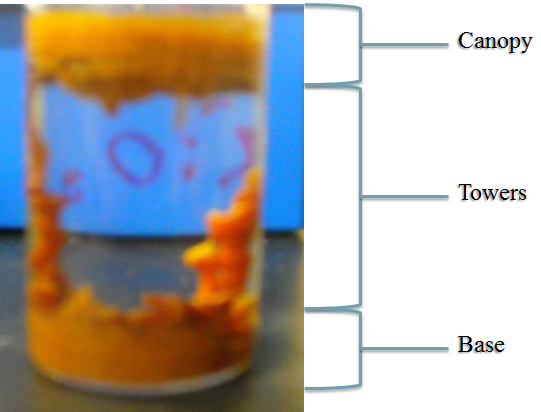
\includegraphics[height=150pt,keepaspectratio]{garden.png}
    \caption{Silica Garden Structures}
\end{scheme} \\


\subsection*{Reversing the Attempt: Backwards Silicate Garden}

\subsection*{Another Interesting System: Vanadia Gardens}

\subsection*{Incorporating Metal into Porous Silica: Nakanishi-Style with Waterglass}

\section*{Conclusions}
Attempts to template mesoporosity onto the structure of silicate gardens via a liquid-crystal templating procedure utilizing cetyltrimethylammonium bromide (CTAB) as a surfactant failed due to the high speed of garden growth. In attempted to slow the growth of the garden by reversing the acidity or basicity, respectively, of the salt crystal and the solution, the growth of the garden was excessively slow, in that the garden could not be differentiated from a selective precipitation of silica onto the salt crystal due to a thermodynamic effect of the salt crystal surface. \\
The discovery of the vanadia garden, which came about as an observation of the general principles expressed by the silicate gardens, allowed for the testing of specific properties in the silica garden system such as the effect of pH and solution density on garden structure. The vanadia garden could be forced to grow towers by acidifying the solution and increasing the amount of metal salt used. \\
Attempting to incorporate metal salts into a macroporous silica system by utilizing a Nakanishi-style synthesis with waterglass ultimately provided inconclusive, as the metal salt was clearly shown to have incorporated itself into the structure of the gel but not in any observable fashion on the scanning electron microscope.

\acknowledgement
I would like to express my appreciation to Dr. Andreas Stein and Mr. Nicholas Petkovich of the University of Minnesota Department of Chemistry. Thanks are also due to Stephen Rudisill, Benjamin Wilson and Yuqiang Qian for help in performing some of the laboratory work, as well as the other members of the Stein group. Finally, the Characterization Facility of the University of Minnesota assisted in the performance of SEM and SAXS measurements on several samples throughout the course of this project.


\suppinfo




\bibliography{sample}

\end{document}
